\documentclass[tikz, border=10pt]{standalone}
\usetikzlibrary{shapes.geometric, positioning, arrows.meta}
\usepackage[T1]{fontenc}
\usepackage{xcolor}
\usepackage{amssymb}

\begin{document}


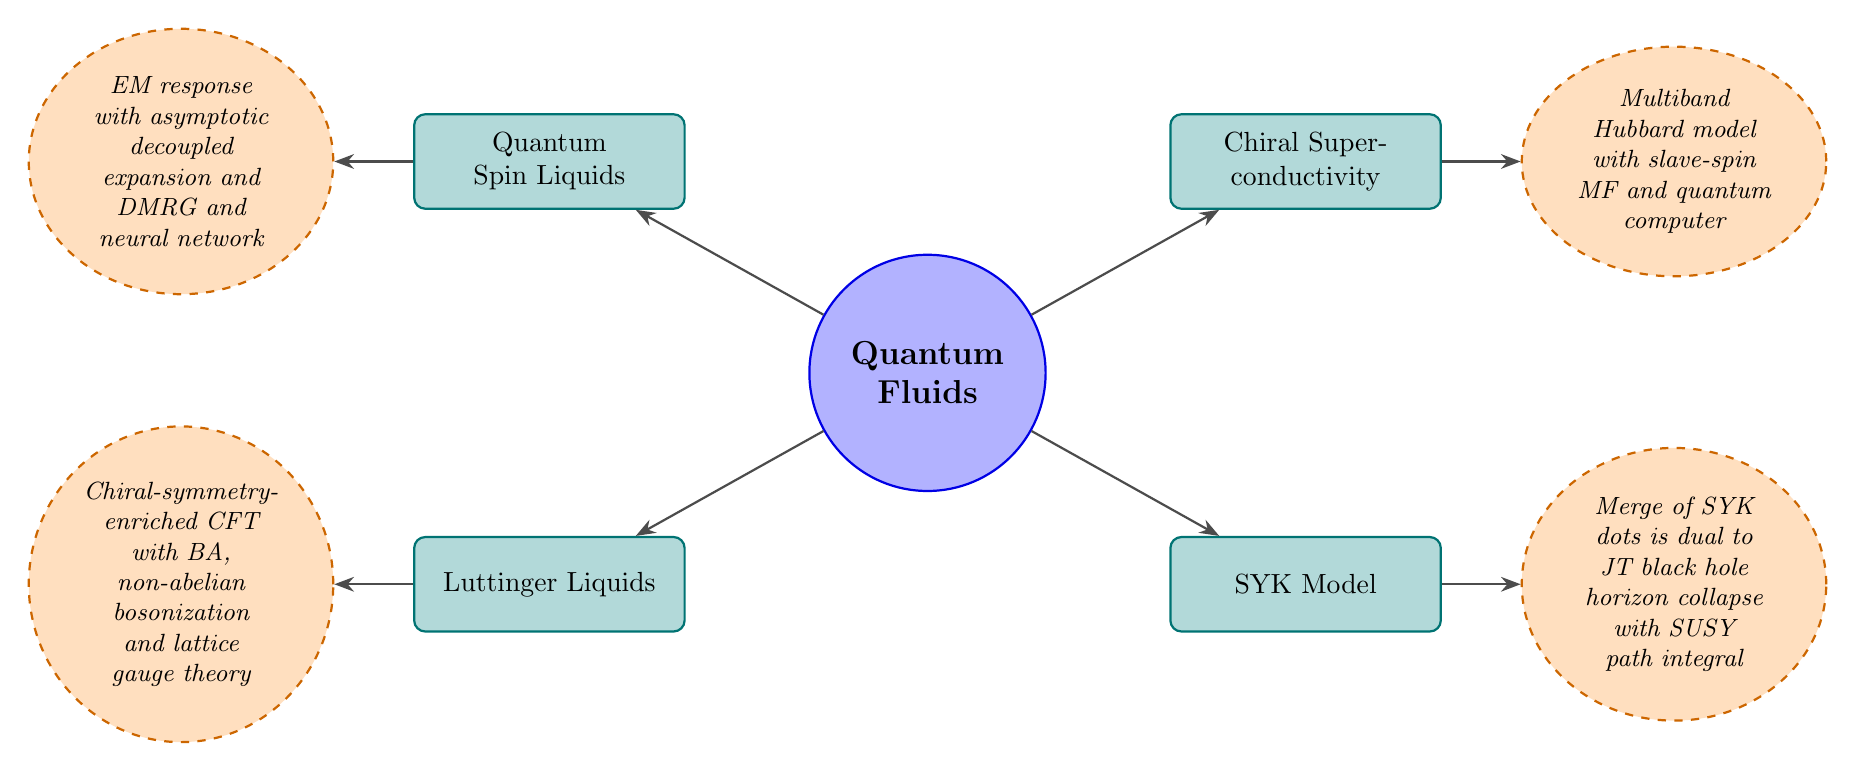
\begin{tikzpicture}[
    node distance=2.5cm and 3cm, % Define vertical and horizontal spacing
    % Style for the central topic
    central_node/.style={
        circle,
        draw=blue!90!black,
        fill=blue!30,
        thick,
        minimum size=3cm,
        text width=2.5cm,
        align=center,
        font=\large\bfseries
    },
    % Style for the main concepts (first layer of bubbles)
    main_concept/.style={
        rectangle,
        rounded corners,
        draw=teal!90!black,
        fill=teal!30,
        thick,
        minimum height=1.2cm,
        text width=3.2cm,
        align=center,
        font=\normalsize
    },
    % Style for the user-editable bubbles (second layer)
    user_bubble/.style={
        ellipse,
        draw=orange!80!black,
        fill=orange!25,
        dashed,
        thick,
        minimum height=1.2cm,
        text width=2.5cm,
        align=center,
        font=\small\itshape
    },
    % Style for the connection lines
    line/.style={
        draw=black!70,
        thick,
        -{Stealth[length=2.5mm]}
    }
]

% --- NODES ---

% Central Node at the origin
\node[central_node] (qf) at (0,0) {Quantum Fluids};

% Main Concepts arranged in a hexagon around the center
\node[main_concept] (sc)  [above right=1cm and 2cm of qf]  {Chiral Superconductivity};
\node[main_concept] (syk) [below right=1cm and 2cm of qf] {SYK Model};
% \node[main_concept] (sf)  [below=of qf]  {Superfluidity};
\node[main_concept] (ll)  [below left=1cm and 2cm of qf]  {Luttinger Liquids};
\node[main_concept] (qsl) [above left=1cm and 2cm of qf] {Quantum Spin Liquids};

% User-Editable Bubbles, positioned relative to their parent concept
\node[user_bubble] (sc_sub)  [right=1cm of sc]  {Multiband Hubbard model with slave-spin MF and quantum computer};
\node[user_bubble] (syk_sub) [right=1cm of syk] {Merge of SYK dots is dual to JT black hole horizon collapse with SUSY path integral};
% \node[user_bubble] (sf_sub)  [below=1cm of sf]  {Deconfined quantum critical point with worm-algo MC};
\node[user_bubble] (ll_sub)  [left=1cm of ll]   {Chiral-symmetry-enriched CFT with BA, non-abelian bosonization and lattice gauge theory};
\node[user_bubble] (qsl_sub) [left=1cm of qsl] {EM response with asymptotic decoupled expansion and DMRG and neural network};


% --- CONNECTIONS ---
% We draw simple, straight lines between the nodes.
\draw[line] (qf) -- (sc);
\draw[line] (qf) -- (syk);
% \draw[line] (qf) -- (sf);
\draw[line] (qf) -- (ll);
\draw[line] (qf) -- (qsl);

\draw[line] (sc) -- (sc_sub);
\draw[line] (syk) -- (syk_sub);
% \draw[line] (sf) -- (sf_sub);
\draw[line] (ll) -- (ll_sub);
\draw[line] (qsl) -- (qsl_sub);

\end{tikzpicture}

\end{document}
